\documentclass{beamer}[10]

\usepackage{graphicx}
\usepackage{xcolor}
\usepackage{tabto}
%\usepackage{beamerthemesplit}
\usepackage{tikz}
\usepackage{cancel}
\usepackage{verbatim}
\usepackage{fancybox}
\usepackage{enumerate}
\usepackage{amsmath,amssymb,amsthm,textcomp,mathtools}
\usepackage[super]{nth}
\usepackage[amssymb]{SIunits}
\usepackage{booktabs}
\usepackage{cancel}
\usepackage{bm}
\usepackage[utf8]{inputenc}
\usepackage{tabularx}
\usepackage{ragged2e}
\newcolumntype{Y}{ >{\RaggedRight\arraybackslash}X}
\usetikzlibrary{arrows,shapes}
\newcommand\T{\rule{0pt}{2.6ex}}
\newcommand\B{\rule[-1.2ex]{0pt}{0pt}}
\definecolor{UUcrimson}{RGB}{204,0,0}
\mode<presentation>
{ \usetheme{default}
  \usecolortheme[named=UUcrimson]{structure}
  \useinnertheme{circles}
  \setbeamercovered{transparent}
  \setbeamertemplate{blocks}[rounded]
  \usefonttheme[onlymath]{serif}
  \setbeamertemplate{navigation symbols}{}
  \setbeamertemplate{footline}[page number]
  \setbeamertemplate{navigation symbols}{}
  \setbeamercolor{section in toc}{fg=black,bg=white}
  \setbeamercolor{alerted text}{fg=UUcrimson!80!gray}
  \setbeamercolor*{palette primary}{fg=white,bg=UUcrimson}
  \setbeamercolor*{palette secondary}{fg=UUcrimson!70!black,bg=gray!15!white}
  \setbeamercolor*{palette tertiary}{bg=UUcrimson!80!black,fg=gray!10!white}
  \setbeamercolor*{palette quaternary}{fg=UUcrimson,bg=gray!5!white}
  \setbeamercolor*{palette sidebar primary}{fg=UUcrimson!10!black}
  \setbeamercolor*{palette sidebar secondary}{fg=white}
  \setbeamercolor*{palette sidebar tertiary}{fg=UUcrimson!50!black}
  \setbeamercolor*{palette sidebar quaternary}{fg=gray!10!white}
  \setbeamercolor{titlelike}{parent=palette primary,fg=white}
  \setbeamercolor{frametitle}{bg=UUcrimson}
  \setbeamercolor{frametitle right}{bg=UUcrimson}
  \setbeamercolor*{separation line}{}
  \setbeamercolor*{fine separation line}{}
}

\usetikzlibrary{backgrounds}
\makeatletter
\tikzstyle{every picture}+=[remember picture]
\tikzset{%
  fancy quotes/.style={
    text width=\fq@width pt,
    align=justify,
    inner sep=1em,
    anchor=north west,
    minimum width=\linewidth,
    font=\itshape
  },
  fancy quotes width/.initial={.8\linewidth},
  fancy quotes marks/.style={
    scale=8,
    text=white,
    inner sep=0pt,
  },
  fancy quotes opening/.style={
    fancy quotes marks,
  },
  fancy quotes closing/.style={
    fancy quotes marks,
  },
  fancy quotes background/.style={
    show background rectangle,
    inner frame xsep=0pt,
    background rectangle/.style={
      fill=gray!25,
      rounded corners,
    },
  }
}
\newenvironment{fancyquotes}[1][]{%
\noindent
\tikzpicture[fancy quotes background]
\node[fancy quotes opening,anchor=north west] (fq@ul) at (0,0) {``};
\tikz@scan@one@point\pgfutil@firstofone(fq@ul.east)
\pgfmathsetmacro{\fq@width}{\linewidth - 2*\pgf@x}
\node[fancy quotes,#1] (fq@txt) at (fq@ul.north west) \bgroup}
{\egroup;
\node[overlay,fancy quotes closing,anchor=east] at (fq@txt.south east) {''};
\endtikzpicture}
\makeatother


\usetikzlibrary{backgrounds}
\makeatletter
\tikzstyle{every picture}+=[remember picture]
\tikzset{%
  fancy defs/.style={
    text width=\fq@width pt,
    align=justify,
    inner sep=0.25em,
    anchor=north west,
    minimum width=\linewidth,
    font=\itshape
  },
  fancy defs width/.initial={.8\linewidth},
  fancy defs marks/.style={
    scale=8,
    text=white,
    inner sep=0pt,
  },
  fancy defs opening/.style={
    fancy defs marks,
  },
  fancy defs closing/.style={
    fancy defs marks,
  },
  fancy defs background/.style={
    show background rectangle,
    inner frame xsep=0pt,
    background rectangle/.style={
      fill=gray!25,
      rounded corners,
    },
  }
}
\newenvironment{fancydefs}[1][]{%
\noindent
\tikzpicture[fancy defs background]
\node[fancy defs opening,anchor=north west] (fq@ul) at (0,0) {};
\tikz@scan@one@point\pgfutil@firstofone(fq@ul.east)
\pgfmathsetmacro{\fq@width}{\linewidth - 2*\pgf@x}
\node[fancy defs,#1] (fq@txt) at (fq@ul.north west) \bgroup}
{\egroup;
\node[overlay,fancy defs closing,anchor=east] at (fq@txt.south east) {};
\endtikzpicture}
\makeatother
\usepackage{scalerel}[2014/03/10]
\usepackage{stackengine}
\usepackage{empheq}
\newcommand*\widefbox[1]{\fbox{\hspace{0.5em}#1\hspace{0.5em}}}

\newcommand\reallywidetilde[1]{\ThisStyle{%
  \setbox0=\hbox{$\SavedStyle#1$}%
  \stackengine{-.1\LMpt}{$\SavedStyle#1$}{%
    \stretchto{\scaleto{\SavedStyle\mkern.2mu\sim}{.5467\wd0}}{.4\ht0}%
%    .2mu is the kern imbalance when clipping white space
%    .5467++++ is \ht/[kerned \wd] aspect ratio for \sim glyph
  }{O}{c}{F}{T}{S}%
}}
\usepackage{media9}

\logo{
\includegraphics[width=0.75cm]{logo.jpg}}
\author[Gibbs]{Dr. Jeremy A. Gibbs}
\institute{Department of Mechanical Engineering\\University of Utah}
\date{Spring 2017}
\title{Environmental Fluid Dynamics: Lecture 4}
% colors
\definecolor{colororange}{HTML}{E65100} % orange
\definecolor{colordgray}{HTML}{795548} % dark gray for note
\definecolor{colorhgray}{HTML}{212121} % heavy dark gray for normal text
\definecolor{colorgreen}{HTML}{009688} % green
\definecolor{colorwhite}{HTML}{FFFFFF} % background white
\definecolor{colorlgray}{HTML}{F5F3EE} % background light gray
\definecolor{colorblue}{HTML}{0277BB} % blue
\definecolor{colorred}{HTML}{CC0000} % red
\newcommand{\fontsizeone}{1.9em}
\setbeamertemplate{caption}{\raggedright\insertcaption\par}
\newcommand{\framecard}[2][colorgreen]{
  {\setbeamercolor{background canvas}{bg=#1}
    \begin{frame}[plain]
    \vfill
    \begin{center}
     {#2}
    \end{center}
    \vfill
    \end{frame}
  }
}

\begin{document}

%----------------------------------------------------------------------------------------
%	TITLE & TOC SLIDES
%----------------------------------------------------------------------------------------

\begin{frame} 
  \titlepage
\end{frame}

%------------------------------------------------

\begin{frame}
\frametitle{Overview}
\tableofcontents
\end{frame}

%------------------------------------------------
\section{Atmospheric Thermodynamics} %
%------------------------------------------------
\framecard[colorred]{{\color{white}\Huge Atmospheric Thermodynamics}}
%------------------------------------------------
\subsection{Air Temperature and Humidy}
%------------------------------------------------

\begin{frame}{Atmospheric Thermodynamics: Air Temperature}
\textbf{Numerous factors influence the vertical distribution of air temperature in the planetary boundary layer (PBL)}. ~\\~\\
Examples:
\begin{itemize}
	\item Type of air mass (and its temperature) overlying the PBL - depends on large-scale systems
	\item Thermal characteristics of surface/sub-surface - affects diurnal range
	\item Net radiation the surface and its vertical distribution - determines warming/cooling of surface and PBL
	\item Sensible heat flux at the surface and its vertical distribution - determines rate of warming/cooling of air due to flux convergence/divergence
\end{itemize}
\end{frame}
%------------------------------------------------

\begin{frame}{Atmospheric Thermodynamics: Air Temperature}
\textbf{Numerous factors influence the vertical distribution of air temperature in the PBL}. ~\\~\\
Examples:
\begin{itemize}
	\item Latent heat fluxes during evaporation and condensation at the surface and in the air - directly influences surface and air temp
	\item Advection of warm of cold air as a function of height in the PBL
	\item Depth of PBL - confines turbulent exchanges over a particular distance 
\end{itemize}
\end{frame}

%------------------------------------------------

\begin{frame}{Atmospheric Thermodynamics: Moisture}
\textbf{Likewise, numerous factors influence the vertical distribution of moisture in the PBL}. ~\\~\\
Examples:
\begin{itemize}
	\item Specific humidity of air mass overlying the PBL
	\item Surface type, temperature, and availability of moisture for evaporation/transpiration
	\item The rate of evapotranspiration or condensation at the surface and vertical distribution of water vapor flux 
\end{itemize}
\end{frame}
%------------------------------------------------

\begin{frame}{Atmospheric Thermodynamics: Moisture}
\textbf{Likewise, numerous factors influence the vertical distribution of moisture in the PBL}. ~\\~\\
Examples:
\begin{itemize}
	\item Variation of horizontal water vapor advection with height
	\item Mean vertical motion in PBL - possibilities of cloud formation and precipitation processes
	\item The depth of the PBL
\end{itemize}
\end{frame}

%------------------------------------------------

\begin{frame}{Atmospheric Thermodynamics: Goal}
\textbf{Goal:} introduce fundamental ideas and relationships in thermodynamics and apply them to situations in the atmosphere
\begin{itemize}
	\item gas laws
	\item hydrostatic equation
	\item first law of thermodynamics
	\item second law of thermodynamics
	\item entropy
\end{itemize}
\end{frame}

%------------------------------------------------
\subsection{Gas Laws}
%------------------------------------------------
\begin{frame}{Atmospheric Thermodynamics: Gas Laws}
\begin{itemize}
	\item Pressure, volume, and temperature of a material are described by an \textbf{equation of state}
	\item All gases generally follows the same equation of state - the \textbf{ideal gas law}
	\item We will assume that atmospheric gases obey this law
	$$pV = mRT$$ where
	\begin{itemize}
		\item $p$ = pressure ($\pascal$)
		\item $V$ = volume ($\metre\cubed$)
		\item $m$ = mass ($\kilo\gram$)
		\item $R$ = gas constant (depends on gas)
		\item $T$ = absolute temperature ($\kelvin$)
	\end{itemize}
\end{itemize}
\end{frame}

%------------------------------------------------
\begin{frame}{Atmospheric Thermodynamics: Gas Laws}
\begin{itemize}
	\item The ideal gas law
	$$pV=mRT$$
	\item Density $\rho = m/V$, so we can rewrite the ideal gas law as 
	$$p = \rho RT$$
	\item We can also introduce specific volume $\alpha = 1/\rho$, which is the volume occupied by unit mass of the gas
	$$p\alpha = RT$$
\end{itemize}
\end{frame}

%------------------------------------------------
\begin{frame}{Atmospheric Thermodynamics: Gas Laws}
$$pV=mRT$$
\begin{itemize}
	\item If $T$ is constant, we get Boyle's Law
	\begin{fancydefs}
		if the temperature of a fixed mass of gas is held constant, the volume of the gas is inversely proportional to its pressure
	\end{fancydefs}
	\item Changes that occur to a body's physical state under constant temperature are called \textit{isothermal}
\end{itemize}
\end{frame}

%------------------------------------------------
\begin{frame}{Atmospheric Thermodynamics: Gas Laws}
$$pV=mRT$$
\begin{itemize}
	\item If $m$ is fixed and $p$ is constant, we get Charles' First Law
	\begin{fancydefs}
		for a fixed mass of gas at constant pressure, the volume of the gas is directly proportional to its absolute temperature
	\end{fancydefs}
	\item If $m$ is fixed and $V$ is constant, we get Charles' Second Law
	\begin{fancydefs}
		for a fixed mass of gas held within a fixed volume, the pressure of the gas is proportional to its absolute temperature
	\end{fancydefs}
	
\end{itemize}
\end{frame}

%------------------------------------------------
\begin{frame}{Atmospheric Thermodynamics: Gas Laws}
\begin{itemize}
	\item Let's define a kilogram-molecular weight (kilomole; $\kilo\mole$) as the molecular mass $M$ expressed in kilograms
	\item Example: the molecular weight of water is 18.015, so $1\ \kilo\mole = 18.015\ \kilo\gram$
	\item The number of moles $n$ in mass $m$ [$\kilo\gram$] is given by
	$$n = \frac{m}{M}$$
\end{itemize}
\end{frame}
%------------------------------------------------
\begin{frame}{Atmospheric Thermodynamics: Gas Laws}
\begin{itemize}
	\item Masses contained in 1 $\mole$ of different substances have same ratios to each other as the molecular weights of the substances
	\item Thus, 1 $\mole$ of a subtance contains same numbers of molecules as 1 $\mole$ of another substance
	\item \textit{i.e.}, the number of molecules in 1 $\mole$ of a substance is a universal constant
	\item \textit{Avagadro's number} = $6.022 \times 10^{23}$ per mole
	\item \textit{Avagadro's hypothesis}
	\begin{fancydefs}
		Gases containing the same number of molecules
		occupy the same volumes at the same temperature
		and pressure
	\end{fancydefs}
\end{itemize}
\end{frame}

%------------------------------------------------
\begin{frame}{Atmospheric Thermodynamics: Gas Laws}
\textbf{Dry Air}
\begin{itemize}
	\item We can use the apparent molecular weight of dry air (total mass of the constituent gases in dry air divided by the total number of moles of the constituent gases)
	$$M_d = \frac{\sum_i m_i}{\sum_i \frac{m_i}{M_i}} = 29\ \kilo\gram\ \kilo\reciprocal\mole$$
	to obtain the gas constant for dry air
	$$R_d = \frac{R_u}{M_d} = \frac{8314}{29} = 287\ \joule\ \reciprocal\kelvin\ \kilo\reciprocal\gram$$
\end{itemize}
\end{frame}
%------------------------------------------------
\begin{frame}{Atmospheric Thermodynamics: Gas Laws}
\textbf{Dry Air}
\begin{itemize}
	\item Why $29 \ \kilo\gram\ \kilo\reciprocal\mole$ for dry air?
	\begin{table}
	\begin{tabular}{c c c c}
	\hline\hline
	\textbf{Component} & \textbf{Volume Ratio} & $\mathbf{M_i}$ & \textbf{Molecular Mass}\\
	\hline
	Oxygen	& $0.2095$ & $32.00$	 & $6.704$\\
	Nitrogen & $0.7809$ & $28.02$ & $21.88$\\
	Carbon Dioxide & $3\times10^{-4}$ & $44.01$ & $0.013$\\
	Hydrogen & $5\times10^{-7}$	 & $2.02$	& $0$\\
	Argon & $9.3\times10^{-3}$ & $39.94$ & $0.373$\\
	Neon &	$1.8\times10^{-5}$ & $20.18$	 & $0$\\
	Helium & $5\times10^{-6}$ & $4.00$	 & $0$\\
	Krypton	& $1\times10^{-4}$ & $83.8$ & $0$\\
	Xenon & $9\times10^{-8}$ & $131.29$ & $0$\\
	\hline
	\multicolumn{3}{c}{\textbf{Apparent Molecular Weight} $\mathbf{M_d}$} & $\mathbf{28.97}$\\
	\hline\hline
	\end{tabular}	
	\end{table}

\end{itemize}
\end{frame}
%------------------------------------------------
\begin{frame}{Atmospheric Thermodynamics: Gas Laws}
\textbf{Water Vapor}
\begin{itemize}
	\item We can apply to individual components of air, for instance water vapor
	$$e \alpha_v = R_vT$$
	where
	\begin{itemize}
		\item $e$ = water vapor pressure
		\item $\alpha_v$ = specific volume of water vapor
		\item $R_v$ is the gas constant for water vapor
	\end{itemize}
	\item Since molecular weight of water is $M_w = 18.016$, then
	$$R_v = \frac{R_u}{M_w} = \frac{8314}{18.016} = 461.5\ \joule\ \reciprocal\kelvin\ \kilo\reciprocal\gram$$ 
	\end{itemize}
\end{frame}

%------------------------------------------------
\begin{frame}{Atmospheric Thermodynamics: Gas Laws}
\begin{itemize}
	\item We can combine the two expressions to show that
	$$\frac{R_d}{R_v} = \frac{M_w}{M_d} \equiv \epsilon = 0.622$$
	\item Since air is a mixture of gases, it follows Dalton's Law of Partial Pressures
	\begin{fancydefs}
		the total pressure exerted by a mixture of gases 
		that do not interact chemically is equal to the
		sum of the partial pressures of the gases
		$$p = \sum_i p_i$$
	\end{fancydefs}
	\end{itemize}
\end{frame}

%------------------------------------------------
\begin{frame}{Atmospheric Thermodynamics: Gas Laws}
\textbf{Moist Air}
\begin{itemize}
	\item Moist air has a smaller molecular weight than dry air
	\item Thus, moist air will have a larger gas constant than dry air
	\item it is inconvenient, however, to use the gas constant for moist air because it depends on amount of water vapor in air (variable, hard to measure)
	\item Optional idea is to use $R_d$ with an ad-hoc temperature variable that accounts for moisture effects
	\item We will call this \textbf{virtual temperature}
	\end{itemize}
\end{frame}

%------------------------------------------------
\begin{frame}{Atmospheric Thermodynamics: Gas Laws}
\textbf{Virtual Temperature}
\begin{itemize}
	\item The density of moist air is given by
	$$\rho = \frac{m_d + m_v}{V} = \rho_d^\prime + \rho_v^\prime$$
	where
	\begin{itemize}
		\item $\rho_d^\prime$ = density that the mass of dry air would have if occupied all of the volume
		\item $\rho_v^\prime$ = density that the mass of moist air would have if occupied all of the volume
		\item We call these partial densities
	\end{itemize}
	\item Note: moist air is less dense than dry air!
	\end{itemize}
\end{frame}

%------------------------------------------------
\begin{frame}{Atmospheric Thermodynamics: Gas Laws}
\textbf{Virtual Temperature}
\begin{itemize}
	\item Gas law for dry air and water vapor
	\begin{align*}
	e &= \rho_v^\prime R_vT\\
	p_d^\prime &= \rho_d^\prime R_d T
	\end{align*}
	$e$ and $p_d^\prime$ are partial pressures.
	\item From Dalton's Law
	$$p = p_d^\prime + e$$
	\item Recall that 
	$$\rho = \rho_d^\prime + \rho_v^\prime$$
	\end{itemize}
\end{frame}

%------------------------------------------------
\begin{frame}{Atmospheric Thermodynamics: Gas Laws}
\textbf{Virtual Temperature}
\begin{itemize}
	\item Combine these expressions
	\begin{align*}
		\rho &= \rho_d^\prime + \rho_v^\prime\\
		\rho &= \frac{p_d^\prime}{R_dT} + \frac{e}{R_vT}\\
		\rho &= \frac{p-e}{R_dT} + \frac{e}{R_vT}\\
		\rho &= \frac{p}{R_dT}\left[1 - \frac{e}{p}(1-\epsilon)\right]
	\end{align*}
	This can be rewritten as
	$$p = \rho R_dT_v$$
	where
	$$T_v \equiv \frac{T}{1 - \frac{e}{p}(1-\epsilon)}$$
\end{itemize}
\end{frame}

%------------------------------------------------
\begin{frame}{Atmospheric Thermodynamics: Gas Laws}
\textbf{Virtual Temperature}
\begin{fancydefs}
the virtual temperature is the temperature that dry air would need to attain in order to have the same density as the moist air at the same pressure	
\end{fancydefs}
\begin{itemize}
	\item Recall that moist air is less dense than dry air for the same $T$ and $p$
	\item Thus, $T_v$ is always greater than $T$
	\item In the case of a very warm and moist air, $T_v$ is only slightly larger than $T$
	\end{itemize}
\end{frame}

%------------------------------------------------
\subsection{Hydrostatic Equation}
%------------------------------------------------
\begin{frame}{Atmospheric Thermodynamics: Hydrostatic Equation}
\textbf{Pressure}
\begin{itemize}
	\item Atmospheric pressure at a given height is the due to the weight of the air overlying that height
	\item Thus, pressure decreases with increasing altitude
	\item For a thin slice of air, there is upward pressure exerted by pressure gradient force (high to low pressure)
	\item This is generally close in magnitude to the downward force caused by gravitational acceleration
	\item If upward = downward, then we say that the atmosphere is in \textit{hydrostatic balance}
	\end{itemize}
\end{frame}
%------------------------------------------------
\begin{frame}{Atmospheric Thermodynamics: Hydrostatic Equation}
\begin{columns}[T]
    \begin{column}{.5\textwidth}
    \begin{minipage}[c][0.8\textheight][c]{\linewidth}
    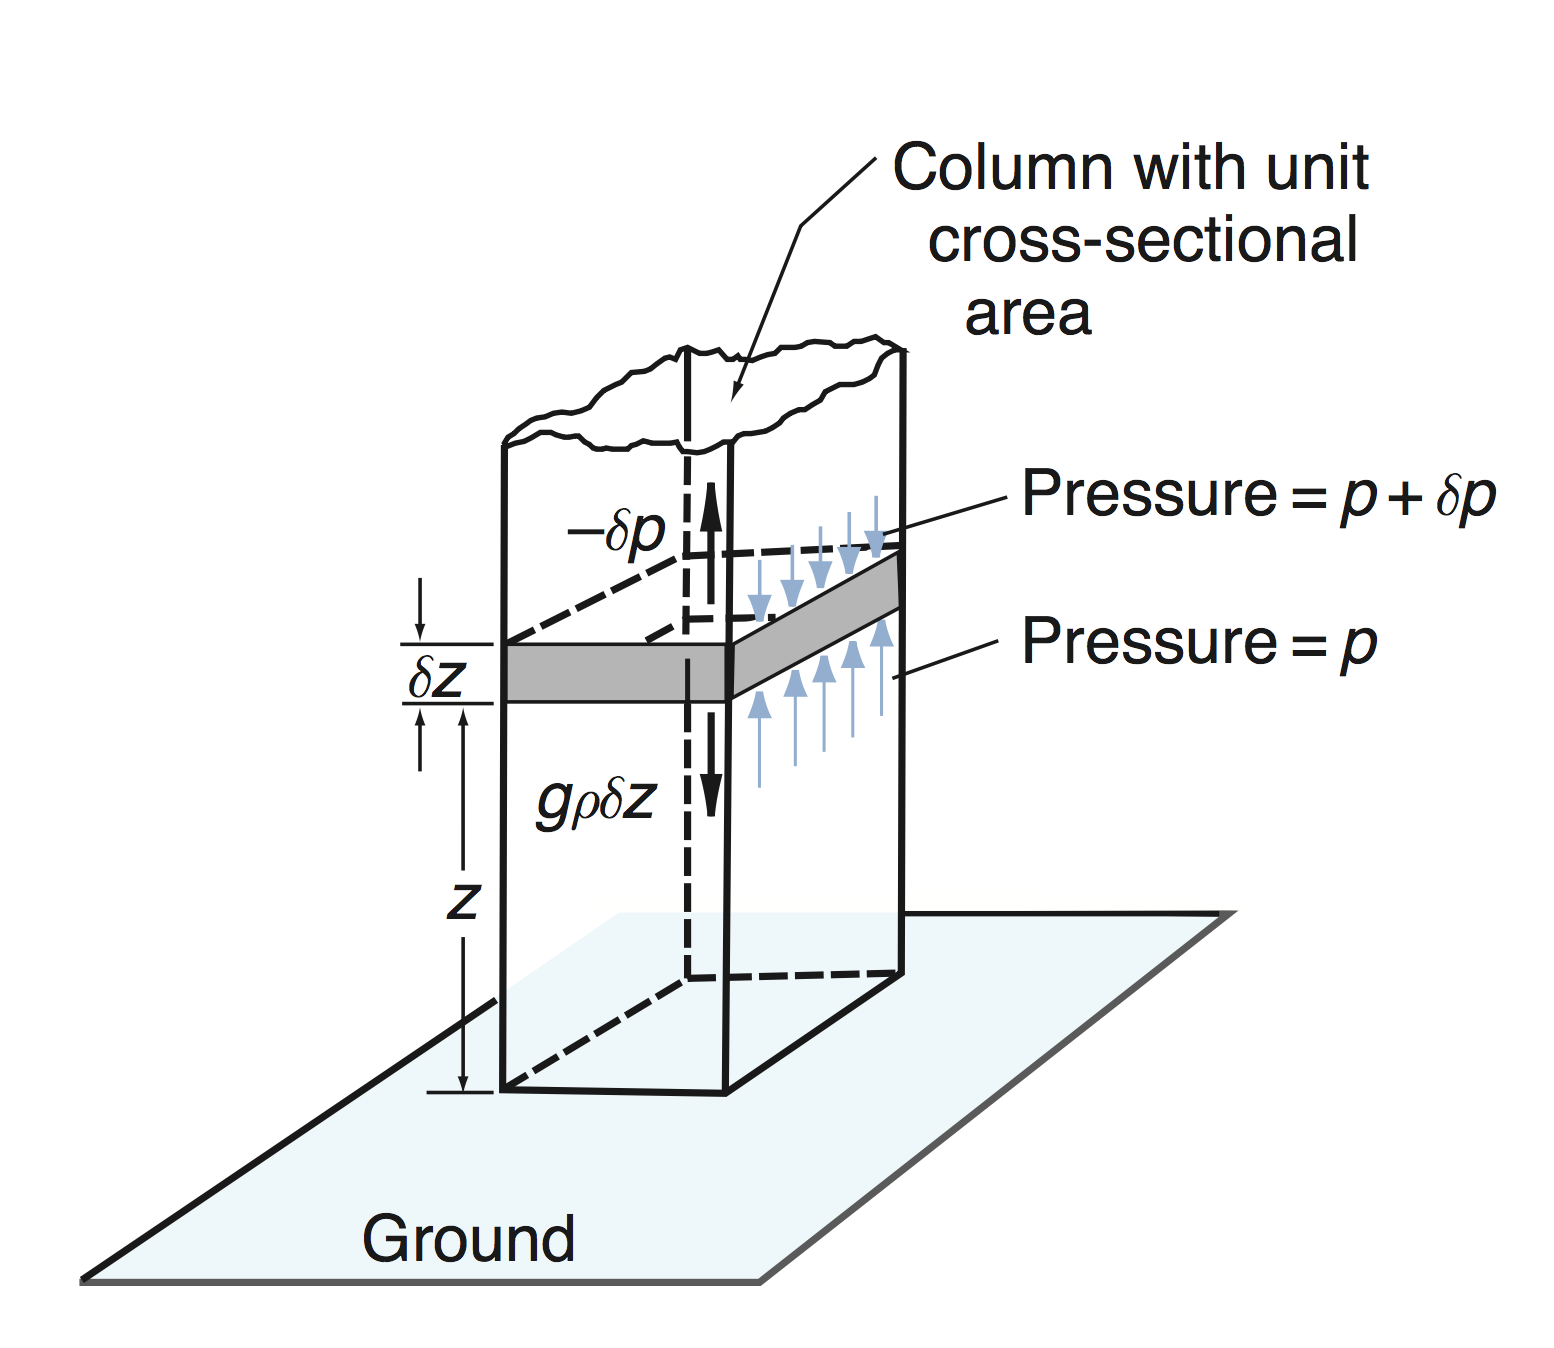
\includegraphics[width=1\textwidth]{fig1.png}\\
    \centering \small From Wallace and Hobbs (2006)
    \end{minipage}
    \end{column}
    \begin{column}{.5\textwidth}
    \begin{minipage}[c][0.8\textheight][c]{\linewidth}
   \begin{itemize}
   	\item Consider column of air w/unit cross-sectional area
   	\item Mass of air between $z$ and $z+\delta z$ is $\rho \delta z$
   	\item Downward force due to gravity is $g\rho \delta z$
   \end{itemize}
      \end{minipage}
    \end{column}
  \end{columns} 
\end{frame}
%------------------------------------------------
\begin{frame}{Atmospheric Thermodynamics: Hydrostatic Equation}
\begin{columns}[T]
    \begin{column}{.5\textwidth}
    \begin{minipage}[c][0.8\textheight][c]{\linewidth}
    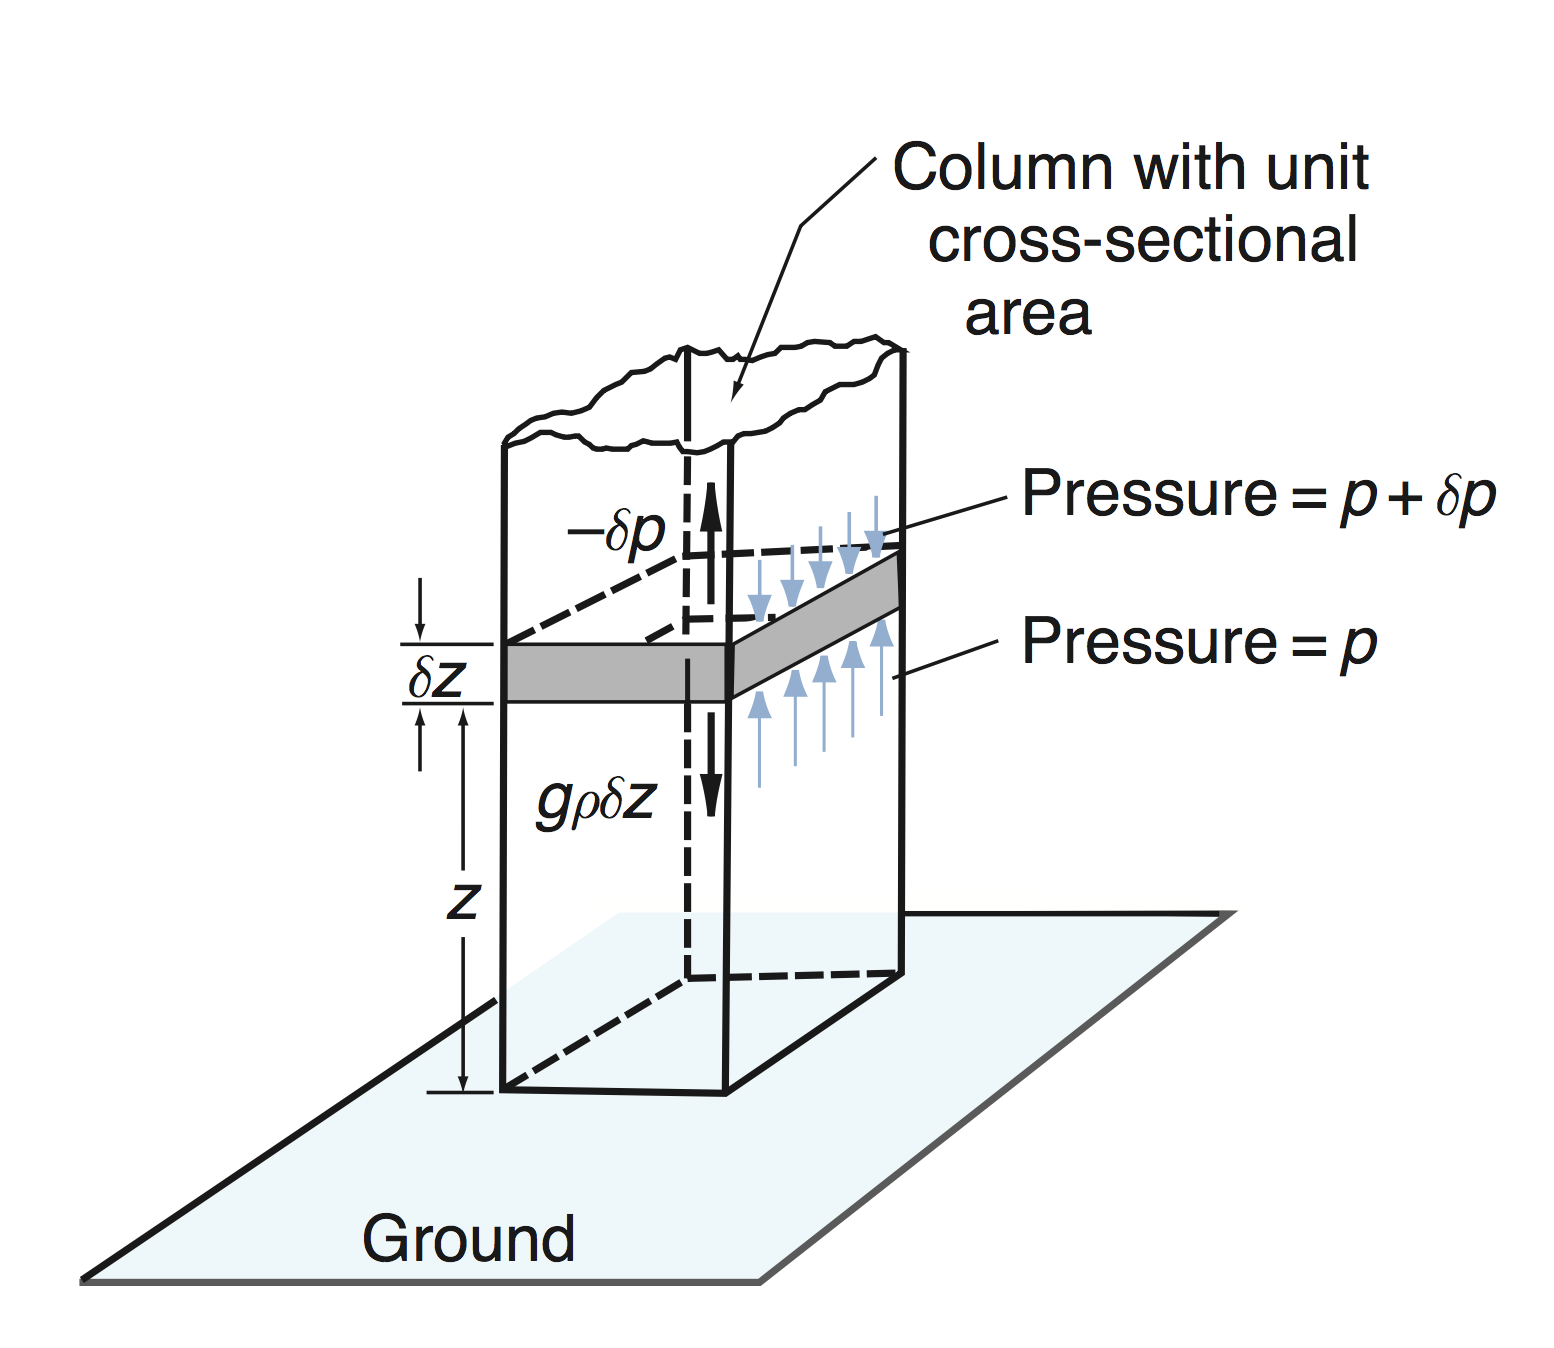
\includegraphics[width=1\textwidth]{fig1.png}\\
    \centering \small From Wallace and Hobbs (2006)
    \end{minipage}
    \end{column}
    \begin{column}{.5\textwidth}
    \begin{minipage}[c][0.8\textheight][c]{\linewidth}
   \begin{itemize}
   	\item Change in pressure between $z$ and $\delta z$ is $\delta p$
   	\item Since pressure decreases with height, $\delta p < 0$, and upward force on bottom is slight bigger than downward force on top
   	\item Thus, net vertical force due to pressure is $-\delta p$
   \end{itemize}
      \end{minipage}
    \end{column}
  \end{columns} 
\end{frame}
%------------------------------------------------
\begin{frame}{Atmospheric Thermodynamics: Hydrostatic Equation}
\begin{columns}[T]
    \begin{column}{.5\textwidth}
    \begin{minipage}[c][0.8\textheight][c]{\linewidth}
    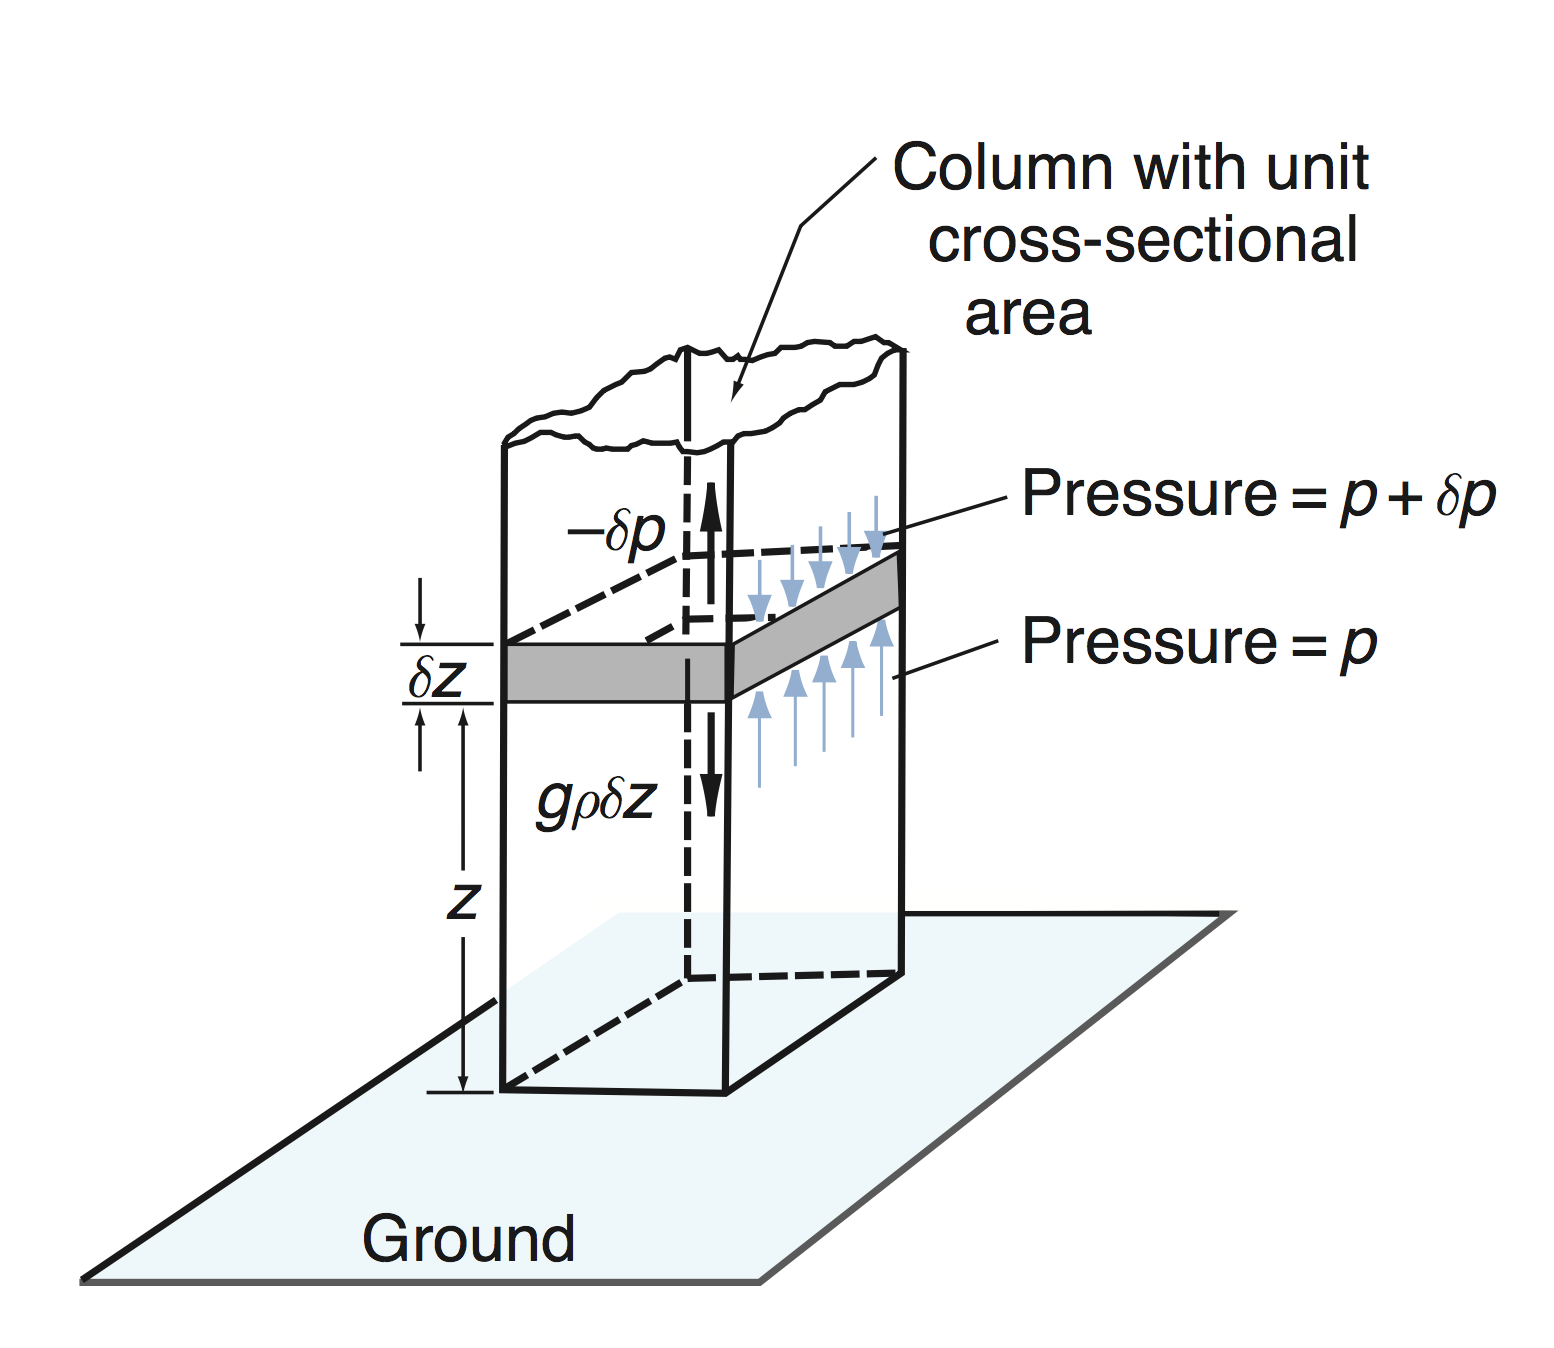
\includegraphics[width=1\textwidth]{fig1.png}\\
    \centering \small From Wallace and Hobbs (2006)
    \end{minipage}
    \end{column}
    \begin{column}{.5\textwidth}
    \begin{minipage}[c][0.8\textheight][c]{\linewidth}
   \begin{itemize}
   	\item If in hydrostatic balance
   	$$-\delta p = g\rho\delta z$$
   	or in limit of $\delta z \rightarrow 0$
   	$$\frac{\partial p}{\partial z} = -\rho g$$
   	the so-called \textbf{hydrostatic equation}
   \end{itemize}
      \end{minipage}
    \end{column}
  \end{columns} 
\end{frame}
%------------------------------------------------
\begin{frame}{Atmospheric Thermodynamics: Hydrostatic Equation}
$$\partial p/\partial z = -\rho g$$
\vspace{-10pt}
\begin{itemize}
	\item Above a fixed point on Earth
	$$-\int^{p(\infty)}_{p(z)} dp = \int^{\infty}_{z} \rho g dz$$
	Since $p(\infty)=0$, we have
	$$p(z) = \int^{\infty}_{z} \rho g dz$$
	\item Thus, the pressure at height $z$ is the weight of the air in the vertical column above it
	\item The ideal sea level pressure (assumes mass of atmosphere distributed evenly) is $1.013\times 10^5\ \pascal = 1013\ \hecto\pascal$ - $1\ atmsophere$
	\end{itemize}
\end{frame}
%------------------------------------------------
\begin{frame}{Atmospheric Thermodynamics: Hydrostatic Equation}
\textbf{Geopotential}
\begin{fancydefs}
	at a point it is the work required to be done against gravity to raise a mass of 1 $\kilo\gram$ from seal level to that point
\end{fancydefs}
\begin{itemize}
	\item In other words, the geopotential $\Phi$ is the gravitational potential per unit mass
	\item Units = [$\joule\ \kilo\reciprocal\gram$] or [$\metre\squared \second\rpsquared$]
	\end{itemize}
\end{frame}
%------------------------------------------------
\begin{frame}{Atmospheric Thermodynamics: Hydrostatic Equation}
\textbf{Geopotential}
\begin{itemize}
	\item Force acting on 1 $\kilo\gram$ at height $z$ is equal to $g$
	\item Thus, work required to raise that from $z$ to $z+dz$ is $gdz$
	\item Accordingly
	$$d\Phi \equiv gdz$$
	\item So, the geopotential at a given height is
	$$\Phi(z) = \int^{z}_0 gdz$$
	\end{itemize}
\end{frame}
%------------------------------------------------
\begin{frame}{Atmospheric Thermodynamics: Hydrostatic Equation}
\textbf{Geopotential}
\begin{itemize}
	\item We can defined \textbf{geopotential height} as
	$$Z \equiv \frac{\Phi(z)}{g_0} = \frac{1}{g_0}\int^{z}_{0} gdz$$
	where $g_0$ is a globally-averaged gravitational acceleration ($9.81\ \metre\ \second\rpsquared$)
	\item Generally in the areas of meteorological importance, $g\approx g_0$ and so $z \approx Z$  
	\end{itemize}
\end{frame}

%------------------------------------------------
\begin{frame}{Atmospheric Thermodynamics: Hydrostatic Equation}
\textbf{Geopotential}
\begin{figure}
	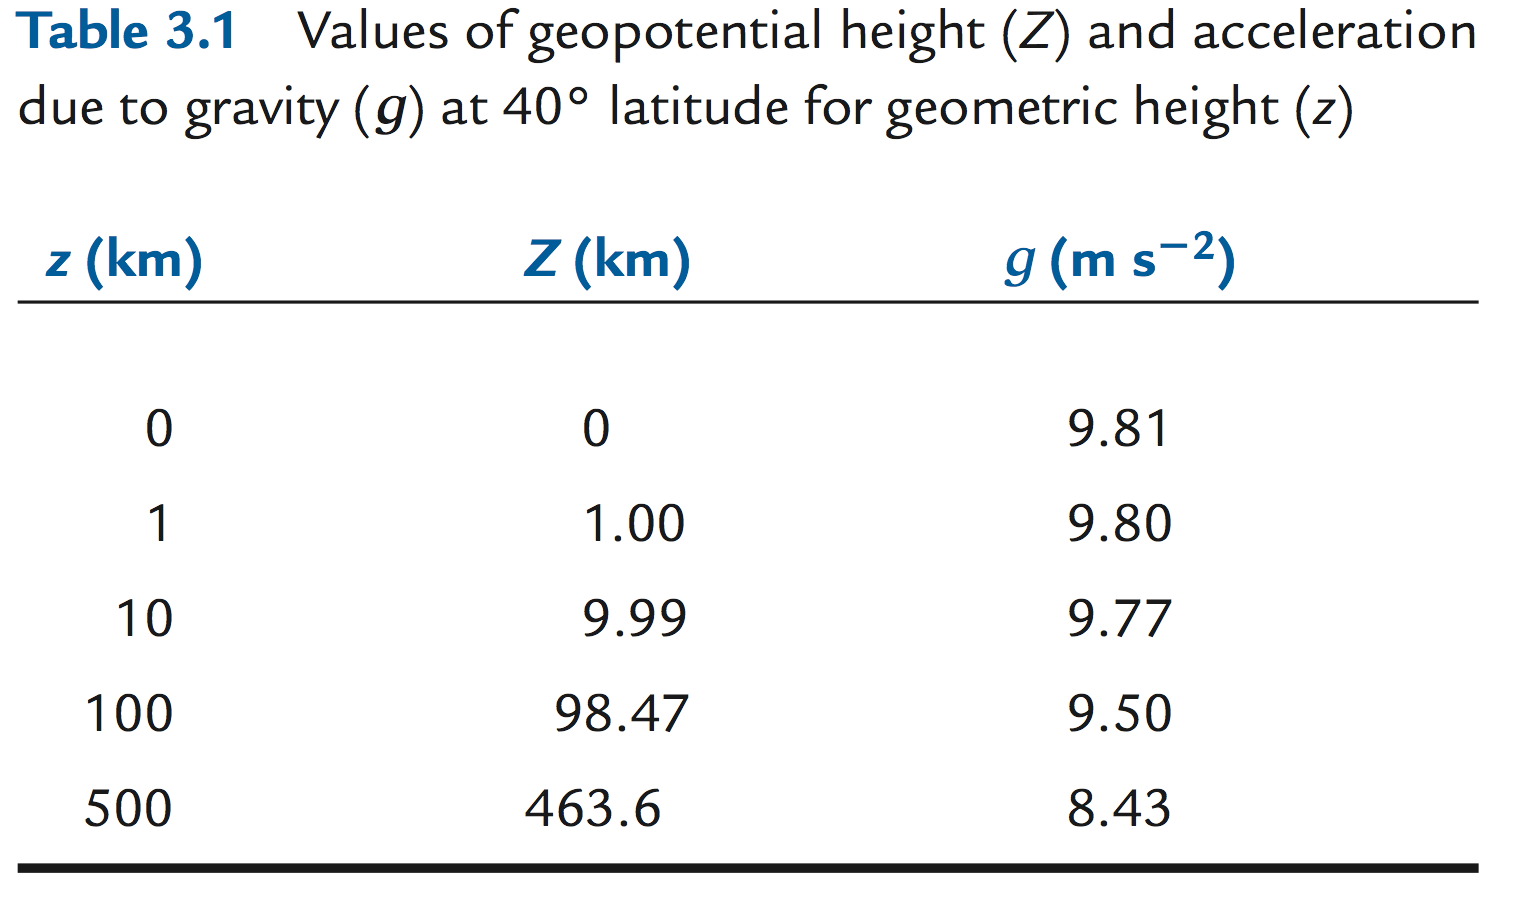
\includegraphics[width=\textwidth]{fig2}
	\centering \small From Wallace and Hobbs (2006)
\end{figure}
\end{frame}

%------------------------------------------------
\begin{frame}{Atmospheric Thermodynamics: Hydrostatic Equation}
\textbf{Geopotential}
\begin{itemize}
	\item Inconvenient to deal with $\rho$.
	$$\frac{\partial p}{\partial z} = -\rho g = -\frac{pg}{RT} = -\frac{pg}{R_dT_v}\Rightarrow gdz = -R_dT_v\frac{dp}{p}$$
	Substitute into geopotential formulation
	$$d\Phi = gdz = -R_dT_v\frac{dp}{p}$$
\end{itemize}
\end{frame}
%------------------------------------------------
\begin{frame}{Atmospheric Thermodynamics: Hydrostatic Equation}
\textbf{Geopotential}
$$d\Phi -R_dT_v\frac{dp}{p}$$
\begin{itemize}
	\item Let's integrate between two pressure levels $p_1$ and $p_2$, with geopotentials $\Phi_1$ and $\Phi_2$
	$$\int^{\Phi_2}_{\Phi_1} = -\int^{p_2}_{p_1} R_d T_v \frac{dp}{p} \Rightarrow \Phi_2 - \Phi_1 = -R_d \int^{p_2}_{p_1} T_v \frac{dp}{p}$$
	\item Divide by $g_0$ and reverse limits of integration
	$$\frac{\Phi_2}{g_0} - \frac{\Phi_1}{g_0} = \frac{R_d}{g_0} \int^{p_1}_{p_2} T_v \frac{dp}{p}\Rightarrow Z_2 - Z_1 = \frac{R_d}{g_0} \int^{p_1}_{p_2} T_v \frac{dp}{p}$$
	\item $Z_2 - Z_1$ is called the \textbf{geopotential thickness} between levels $p_2$ and $p_1$
\end{itemize}
\end{frame}

%------------------------------------------------


\end{document}

